\documentclass[../mathNotesPreamble]{subfiles}

\providecommand{\relscalefact}{1.4}
\begin{document}
\relscale{\relscalefact}
  \section{5.2: Logarithmic Functions and Their Properties}
    \begin{defn*}
      \begin{align*}
        \intertext{For $a>0$ and $a\neq 1$, the \textbf{logarithmic function}}
        y&=\log_a(x) \tag{logarithmic form}
        \intertext{has domain $x>0$, base $a$, and is defined by}
        a^y&=x \tag{exponential form}
      \end{align*}
    \end{defn*}

    \begin{ex*}
      Rewrite the following in exponential form
    \end{ex*}
    \begin{extasks}[after-item-skip=\stretch{1}](2)
      \task $4=\log_2(16)$
      \task $5=\log_{10}(100,000)$
      \task $\frac{1}{2}=\log_{16}(4)$
      \task $\mathllap{-}4=\log_3\parens{\frac{1}{81}}$
      \task $\mathllap{-}\frac{1}{4}=\log_{625}\parens{\frac{1}{5}}$
      \task $\mathllap{-}\frac{5}{3}=\log_\frac{1}{8}(32)$
    \end{extasks}
    \vspace*{\stretch{1}}
    \pagebreak


    \begin{ex*}
      %simplify expressions
      Simplify the following:
    \end{ex*}
    \begin{extasks}[after-item-skip=\stretch{1}](2)
      \task $\log_3(9)$
      \task $\log_4(2)$
    \end{extasks}
    \vspace*{\stretch{1}}
    \begin{ex*}
      Solve the following:
    \end{ex*}
    \begin{extasks}[after-item-skip=\stretch{1}](2)
      \task $\log_{5}(x)=4$
      \task $\log_{8}(x)=1$
      \task $\log_{81}(x)=-\frac{1}{4}$
      \task $\log_{10}(x+4)=3$
    \end{extasks}
    \vspace*{\stretch{1}}
    \pagebreak

    \begin{center}
      \fbox{\parbox{0.5\linewidth}{
        \begin{tabular}{ll}
          \textbf{Common logarithms:}& $\log(x)=\log_{10}(x)$\\
          \textbf{Natural logarithms:}& $\phantom{\log(x)}\mathllap{\ln(x)}=\log_{e}(x)$
        \end{tabular}
      }}
    \end{center}

    \begin{ex*}[The Rule of 70]
      %rule of 70 (p331)
      If $\$P$ is invested for $t$ years at interest rate $r$, compounded continuously, then the future value of the investment is given by
        \[S=Pe^{rt}.\]
      Find the value of $t$ when the investment doubles.
    \end{ex*}
    \pagebreak

    \begin{center}
      \fbox{\parbox{0.75\linewidth}{
        \textbf{Change of base formula:}\\
        If $a>0$, $b>0$ with $a\neq 1$ and $b\neq 1$, then
          \[\log_b(x)=\frac{\log_a(x)}{\log_a(b)}.\]
        \emph{Note}: This works for any valid base!
          \[\textnormal{Base } e: \quad \log_b(x)=\frac{\ln(x)}{\ln(b)} \hspace*{15mm} \textnormal{Base } 10: \quad \log_b(x)=\frac{\log(x)}{\log(b)}\]
      }}
    \end{center}
    \begin{ex*}
      Solve the following
    \end{ex*}
    \begin{extasks}[after-item-skip=\stretch{1}](2)
      \task $3^x=10$
      \task $6.5^x=5$
    \end{extasks}
    \vspace*{\stretch{1}}
    \pagebreak

    \begin{ex*}
      Fill in the tables below and graph $a^x$ and $\log_a(x)$ on the same axes.
    \end{ex*}
    \noindent
    \hspace*{\stretch{1}}
    \begin{minipage}{0.4\linewidth}
      \renewcommand{\arraystretch}{1.5}
      \begin{center}
        \begin{tabular}{@{}rr@{}}\toprule
          $x$& $y=a^x$\\\toprule
          -2& \\
          -1& \\
          0& \\
          1& \\
          2& \\
        \end{tabular}
        \hspace*{\stretch{1}}
        \begin{tabular}{@{}rr@{}}\toprule
          $x$& $y=\log_a(x)$\\\toprule
          &-2\\
          &-1 \\
          &0\\
          &1\\
          &2\\
        \end{tabular}
      \end{center}
    \end{minipage}\hspace*{\stretch{1}}
    \begin{minipage}{0.35\linewidth}
      \begin{flushright}
        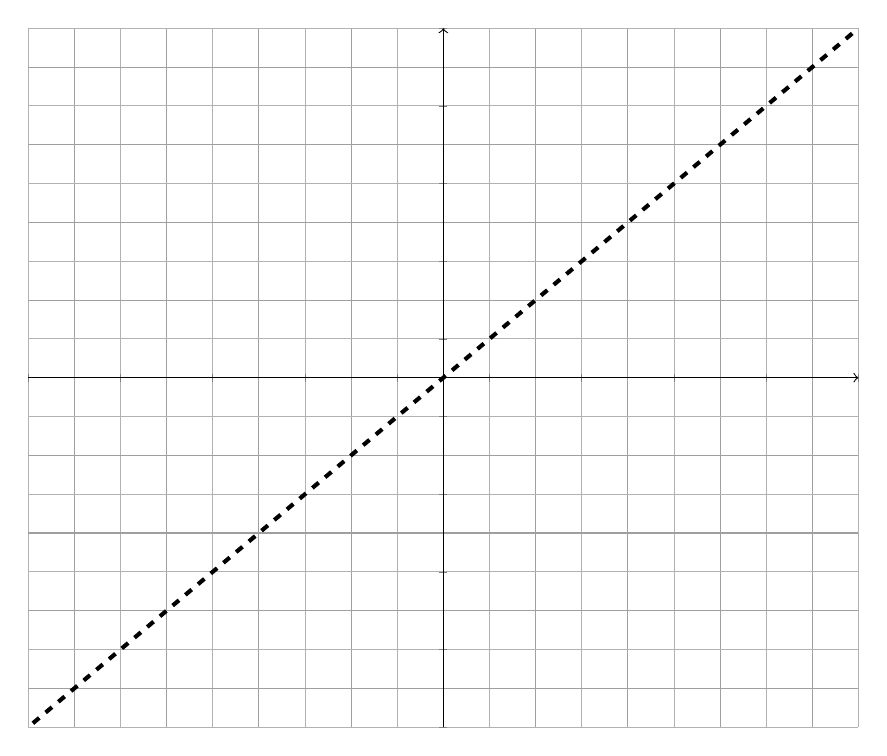
\begin{tikzpicture}[scale=1.0]
          \begin{axis}[
            grid=both, %major,minor
            grid style={line width=0.3pt, draw=gray!60},
            major grid style={line width=0.375pt, draw=gray!75},
            axis lines=center,
            axis line style={black,->},
            xmin=-4.5, xmax=4.5,
            ymin=-4.5, ymax=4.5,
            xmajorticks=false,
            ymajorticks=false,
            minor x tick num=1,
            minor y tick num=1,
            enlargelimits={value=0.5, auto},
            ticklabel style={font=\footnotesize,inner sep=0.5pt,fill=white,opacity=1.0, text opacity=1},
            width=\linewidth
            ]
              \addplot[-, dashed, black, line width=1.5pt]{x};
          \end{axis}
        \end{tikzpicture}\\
        \centering
        \href[pdfnewwindow]{https://www.desmos.com/calculator/fbxvj3gjd7}{\textcolor{blue}{\underline{Try this!}}}
      \end{flushright}
    \end{minipage}
    \vspace*{\stretch{1}}

    \begin{ex*}
      %graph log(x)
      Graph $\log(-x)$
    \end{ex*}
    \hspace*{\stretch{1}}
    \begin{minipage}{0.5\linewidth}
      \begin{flushright}
        
\begin{tikzpicture}[scale=1.0]
          \begin{axis}[
            grid=both, %major,minor
            grid style={line width=0.3pt, draw=gray!60},
            major grid style={line width=0.375pt, draw=gray!75},
            axis lines=center,
            axis line style={black,->},
            xmin=-4.5, xmax=4.5,
            ymin=-4.5, ymax=4.5,
            xmajorticks=false,
            ymajorticks=false,
            minor x tick num=1,
            minor y tick num=1,
            enlargelimits={value=0.5, auto},
            ticklabel style={font=\footnotesize,inner sep=0.5pt,fill=white,opacity=1.0, text opacity=1},
            width=\linewidth
            ]
          \end{axis}
        \end{tikzpicture}
      \end{flushright}
    \end{minipage}
    \vspace*{\stretch{1}}
    \pagebreak

    \begin{ex*}
      %graph log(x)
      Graph $\ln(x)$
    \end{ex*}
    \hspace*{\stretch{1}}
    \begin{minipage}{0.5\linewidth}
      \begin{flushright}
        
\begin{tikzpicture}[scale=1.0]
          \begin{axis}[
            grid=both, %major,minor
            grid style={line width=0.3pt, draw=gray!60},
            major grid style={line width=0.375pt, draw=gray!75},
            axis lines=center,
            axis line style={black,->},
            xmin=-4.5, xmax=4.5,
            ymin=-4.5, ymax=4.5,
            xmajorticks=false,
            ymajorticks=false,
            minor x tick num=1,
            minor y tick num=1,
            enlargelimits={value=0.5, auto},
            ticklabel style={font=\footnotesize,inner sep=0.5pt,fill=white,opacity=1.0, text opacity=1},
            width=\linewidth
            ]
          \end{axis}
        \end{tikzpicture}
      \end{flushright}
    \end{minipage}
    \vspace*{\stretch{1}}

    \begin{ex*}
      %graph log(x)
      Graph $-\log_2(-x)$
    \end{ex*}
    \hspace*{\stretch{1}}
    \begin{minipage}{0.5\linewidth}
      \begin{flushright}
        
\begin{tikzpicture}[scale=1.0]
          \begin{axis}[
            grid=both, %major,minor
            grid style={line width=0.3pt, draw=gray!60},
            major grid style={line width=0.375pt, draw=gray!75},
            axis lines=center,
            axis line style={black,->},
            xmin=-4.5, xmax=4.5,
            ymin=-4.5, ymax=4.5,
            xmajorticks=false,
            ymajorticks=false,
            minor x tick num=1,
            minor y tick num=1,
            enlargelimits={value=0.5, auto},
            ticklabel style={font=\footnotesize,inner sep=0.5pt,fill=white,opacity=1.0, text opacity=1},
            width=\linewidth
            ]
          \end{axis}
        \end{tikzpicture}
      \end{flushright}
    \end{minipage}
    \vspace*{\stretch{1}}
    \pagebreak

    \begin{ex*}
      Evaluate the following:
    \end{ex*}
    \begin{extasks}[after-item-skip=\stretch{1}](2)
      \task $f(x)=\ln(x)$;\quad  $f\parens{e^{-3x}}$
      \task $f(x)=5^x$;\quad $f\parens{\log_5(10)}$
    \end{extasks}
    \vspace*{\stretch{1}}

    \noindent
    \textbf{Properties of exponents and logarithms:} Assume $a>0$:% and $a\neq 1$:
    \begin{center}
      \fbox{\begin{minipage}{0.7\linewidth}
        \begin{align*}
          a^y&=x& \hspace*{20mm}\log_a(x)&=y\\[5mm]
          a^1&=a& \log_a(a)&=1\\[5mm]
          a^0&=1& \log_a(1)&=0\\[5mm]
          a^xa^y&=a^{x+y}& \log_a(xy)&=\log_a(x)+\log_a(y)\\[5mm]
          \dfrac{a^x}{a^y}&=a^{x-y}& \log_a\parens{\frac{x}{y}}&=\log_a(x)-\log_a(y)\\[5mm]
          a^{xy}&=\parens{a^x}^y& \log_a(x^y)&=y\log_a(x)\\[5mm]
          a^{\log_a(x)}&=x& \log_a(a^x)&=x
        \end{align*}
      \end{minipage}}
    \end{center}

  \pagebreak
\end{document}
